\chapter{Systementwurf}
\label{cha:Systementwurf}
In diesem Kapitel geht es um den ersten groben Entwurf des zu entwickelten Roboter. Hierbei wird auf die benötigten Komponenten näher eingegangen. Der Vier Gewinnt spielende Roboter soll mit LEGO SPIKE realisiert werden.  


%Es soll eine detaillierte und funktionsfähige Vorrichtung entworfen werden, die in der Lage ist, Spielsteine präzise und zuverlässig in die vorgesehenen Spalten des Spielständers einzuführen. Dazu muss der Mechanismus so gestaltet sein, dass er unterschiedliche Positionen des Spielständers ansteuern und die Spielsteine mit der nötigen Genauigkeit platzieren kann. Nach dem Einwurf des Spielsteins muss die Vorrichtung den Spielständer wieder für den nächsten Zug freigeben, was eine genaue Steuerung und Rückkehr in die Ausgangsposition erfordert. Die mechanische Konstruktion muss robust und wiederholgenau arbeiten, um einen flüssigen und störungsfreien Spielablauf zu gewährleisten.


\section{Komponenten}
Zur Verwendung stehen folgende Sensorik und Aktorik zur Verfügung:


\begin{itemize}
	\item \textbf{großer LEGO® Technic Hub:}
	Der Hub ist das Steuerungselement des Spike Prime Systems. Er umfasst sechs Ein-/Ausgänge, welche den Anschluss von Peripheriegeräten, wie Sensorik und Aktorik, ermöglicht. Mit einem Micro-USB-Anschluss und Bluetooth wird die Kommunikation mit kompatiblen Endgeräten hergestellt. Der Hub besitzt ein integriertes MicroPython-Betriebssystem mit einem 100-MHz-Prozessor. 
	Weitere Ausstattungen sind:
	Individuell anpassbaren Lichtmatrix (5x5)
	Aufzeigen von wichtigen Informationen und Statusmeldungen
	Tasten
	Ermöglichen eine einfache Navigation und Steuerung durch Menüs 
	Lautsprecher
	6-achsigen Kreiselsensor
	
	\begin{figure}[H]
		\centering
		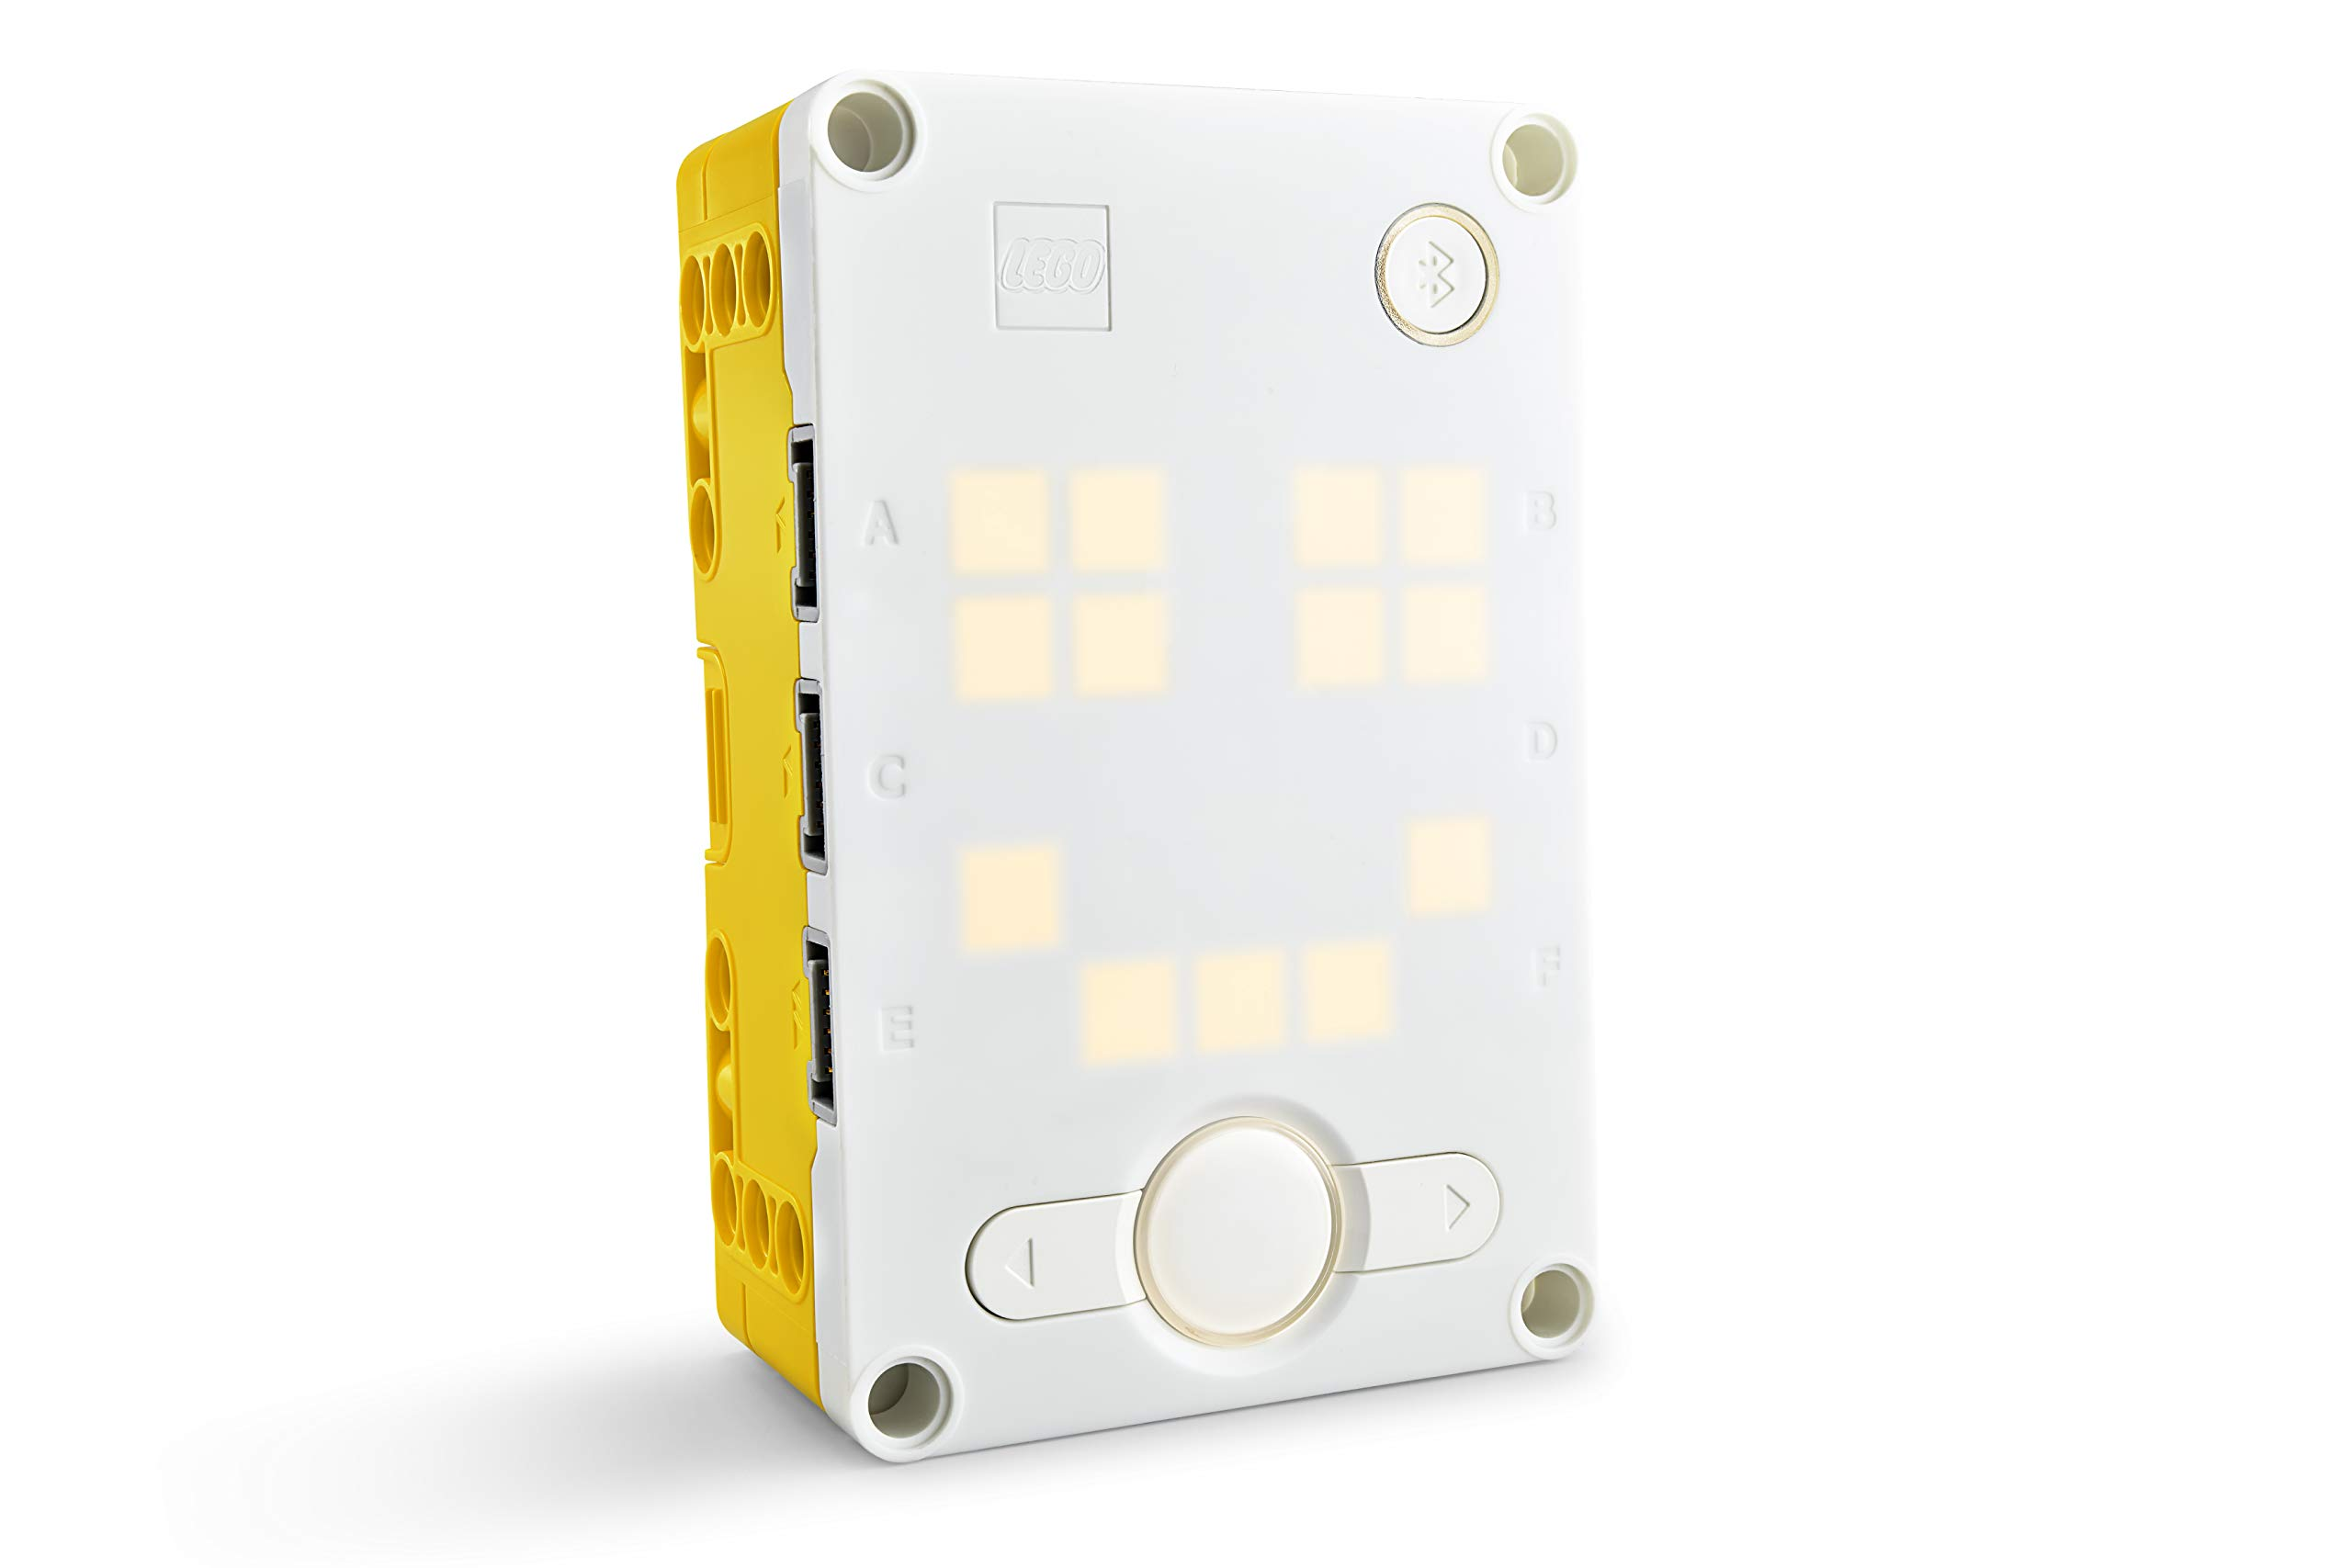
\includegraphics[width=0.5\linewidth]{images/Hub}
		\caption{Lego Technic Hub}
		\label{fig:hub}
	\end{figure}
	
	
	\item \textbf{LEGO® Technic Farbsensor:}
	Dieser Sensor kann durch die Intensität des reflektierten Lichts, welche er durch den eingebauten Lichtring erzeugt, bis zu acht Farben erkennen und unterscheiden (erkennbare Farben: schwarz, blau, rot, weiß, braun, gelb, pink und grün).  Er wird vor allem bei Anwendungen, wie Sortieren nach Farben, Linienverfolgung von farbigen Streifen und zum Ausführen von farbcodierten Befehlen eingesetzt. Um die Farberkennung optimal auf die entsprechende Umgebung anzupassen, wird das Umgebungslicht zuvor ausgewertet.
	
	\begin{figure}[H]
		\centering
		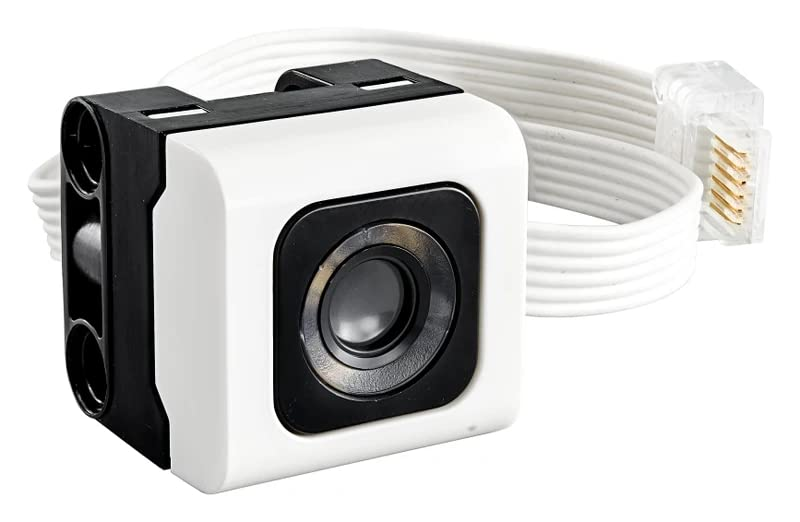
\includegraphics[width=0.5\linewidth]{images/Farbsensor}
		\caption{Lego Technic Farbsensor}
		\label{fig:farbsensor}
	\end{figure}
	
	
	\item \textbf{LEGO® Technic Großer Winkelmotor}
	Für die Bewegungssteuerung wird dieser Winkelmotor mit hoher Drehkraft und präziser Steuerung verwendet. Dieser Motor ist dafür ausgelegt, um schwere und komplexe Konstruktionen exakt in Geschwindigkeit und Position verfahren zu können. Dies wird durch den internen Winkel- und Rotationssensor ermöglicht. Der Anwendungsbereich ist vielseitig, unter anderem wird dies als Antrieb von Rädern, Gelenke, Greifarme, Hebevorrichtungen und Drehscheibe angewandt. Vor allem für Aufgaben, welche eine genau und wiederholbare Aktion ausüben müssen.
	
	\begin{figure}[H]
		\centering
		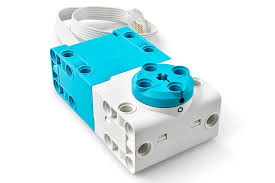
\includegraphics[width=0.5\linewidth]{images/Motor}
		\caption{Lego Technic Winkelmotor}
		\label{fig:motor}
	\end{figure}
	
\end{itemize}

\section{Zusammenspiel von Soft- und Hardware}

Der LEGO SPIKE Farbsensor eignet sich hervorragend zur Erkennung der Spielsteine in einem Vier-Gewinnt-Spiel. 

\subsection{Mechanische Konstruktion des Farbsensor-Systems}

Das Farbsensor-System basiert auf einem zweiachsigen Antriebssystem, das eine präzise Bewegung sowohl in vertikaler als auch in horizontaler Richtung ermöglicht. 

Die \textbf{vertikale Bewegung} wird durch eine Kettenkonstruktion realisiert, an der der Farbsensor befestigt ist. Ein LEGO SPIKE Motor treibt die Kette präzise an und sorgt dafür, dass der Sensor alle sechs Reihen des Spielfeldes abtasten kann. 

Die \textbf{horizontale Bewegung} erfolgt über einen Wagen mit vier Rädern. Dieser Wagen wird durch einen zweiten Motor angetrieben, der mit Encoderwerten für eine präzise Positionierung gesteuert wird. Durch die horizontale Bewegung können alle sieben Spalten des Spielfeldes abgedeckt werden.

Die \textbf{Steuerung der Bewegungen} erfolgt durch eine koordinierte Ansteuerung beider Achsen, wodurch der Farbsensor schrittweise von Position zu Position bewegt wird. Optimierte Verfahrwege minimieren die Scanzeit, und eine Kalibrierung der Positionen gewährleistet eine genaue Ausrichtung des Sensors.

Diese mechanische Konstruktion ermöglicht eine zuverlässige und präzise Abtastung aller 42 Spielfeldpositionen des Vier-Gewinnt-Spiels und stellt somit eine optimale Grundlage für die Umsetzung  dar.
